\chapter{Measurement process and analysis}\label{chap:03}

Prior to data acquisition, comprehensive familiarization with both the hardware setup and Alibava software interface is essential. The measurement sequence initiates with a systematic current-voltage characterization of the sensor, recording leakage current at 10 V intervals from 0 V to 200 V beyond the anticipated depletion voltage. The software-based measurements commence with a \textit{pedestal run} (1000 events) to determine the pedestal and the noise.

Before using the laser or the radioactive source, a set of calibration measurements are started. The first calibration is used to determine the optimal delay. It is started using the \textit{Delay measurement} button in the Alibava software. After this run, five different channels are used in a \textit{Calibration run}, with the applied voltage above the depletion voltage.

Another run is started afterwards with the applied voltage turned down to 0 V.

For laser-based measurements, the laser is lead into the detector unit using the optic fiber cable. It is then synchronized for timing calibration using the \textit{laser sync} function.
Then the structure of the sensor is probed by recording 1000 events at 35 discrete positions (10 μm intervals). Charge Collection Efficiency (CCE) characterization is performed through voltage-dependent measurements (0-200 V in 10 V steps, 1000 events per setting).

Radioactive source measurements follow an analogous protocol but with enhanced statistics: 10,000 events per voltage step during CCE scans. The experiment concludes with a high-statistics source measurement recording 1,000,000 events for large scan analysis.
%----------------------------------------------------%
\newpage
\section{Depletion voltage}

The first measurement of the analysis is the current-voltage characteristic curve of the silicon strip sensor. \autoref{fig:depletion} presents the measured leakage current as a function of applied bias voltage. The characteristic curve exhibits a flattening at 60 V, that corresponds to the depletion voltage $U_{\text{dep}} = 60$ V. To ensure stable operation under full depletion conditions during subsequent measurements, the bias voltage was maintained at 80 V.

\begin{figure}[H]
       %\setkeys{Gin}{draft=false}
	\centering
	\fcolorbox{black}{white}{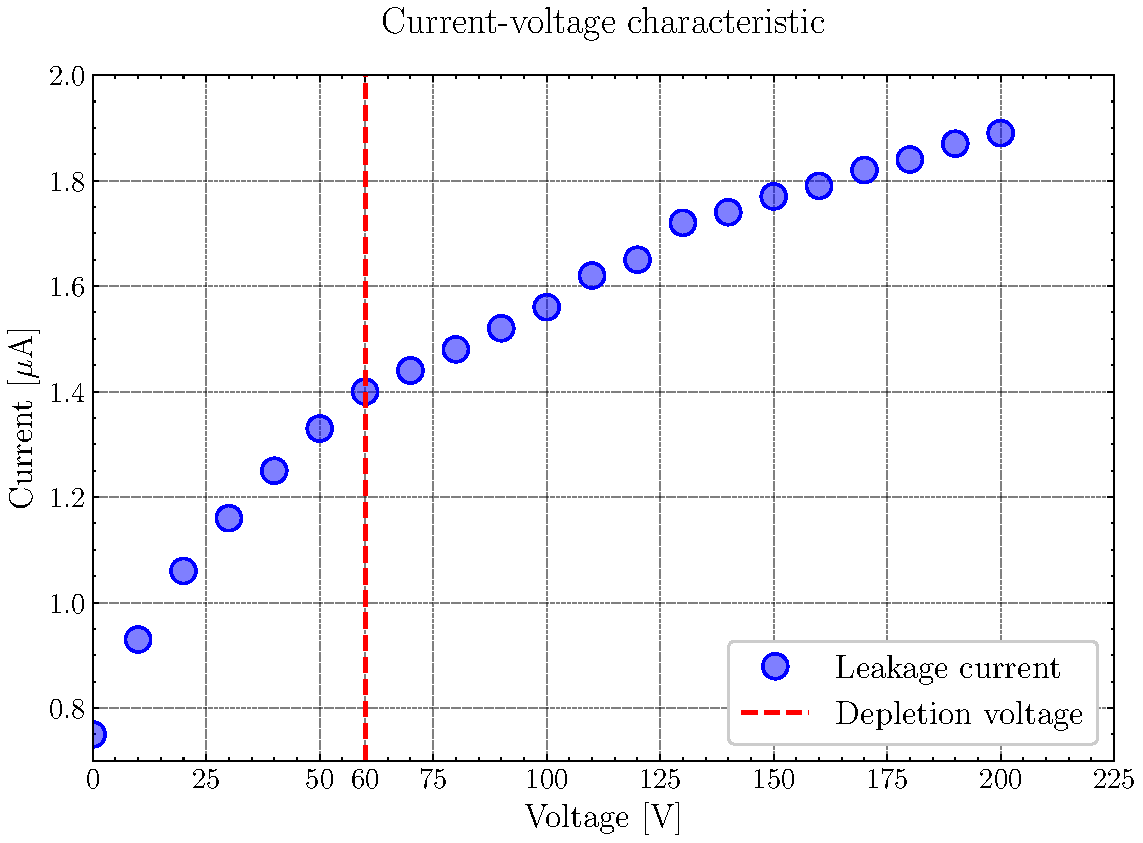
\includegraphics[scale=0.5]{graphs/CurrVoltChar.pdf}}
	\caption{Plot of the measured current-voltage characteristic.}
	\label{fig:depletion}
\end{figure}
%----------------------------------------------------%
\section{Pedestal run}

The pedestal run data provides the basis for quantifying strip detector noise. For each strip, the pedestal value $P(i)$ is computed as the arithmetic mean of ADC counts across all events, consistent with \cref{eq:pedestal}. Subsequent processing determines the common mode shift $D(k)$ for individual events by first subtracting the ADC counts of each
strip and again taking the mean value according to \cref{eq:shift}.

\begin{figure}[H]
       %\setkeys{Gin}{draft=false}
	\centering
	\fcolorbox{black}{white}{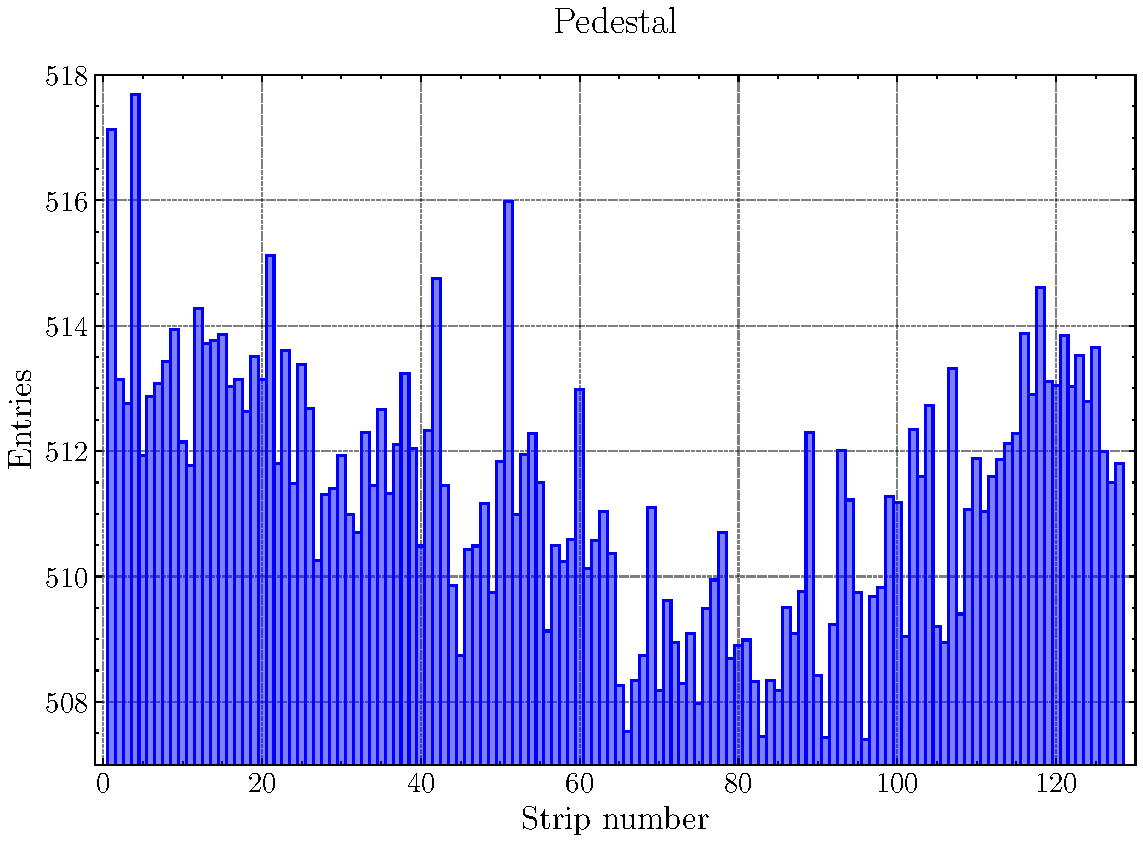
\includegraphics[scale=0.5]{graphs/pedestal.pdf}}
	\caption{Bar diagrams of the pedestal of the 128 individual strips.}
	\label{fig:pedestal}
\end{figure}

\begin{figure}[H]
       %\setkeys{Gin}{draft=false}
	\centering
	\fcolorbox{black}{white}{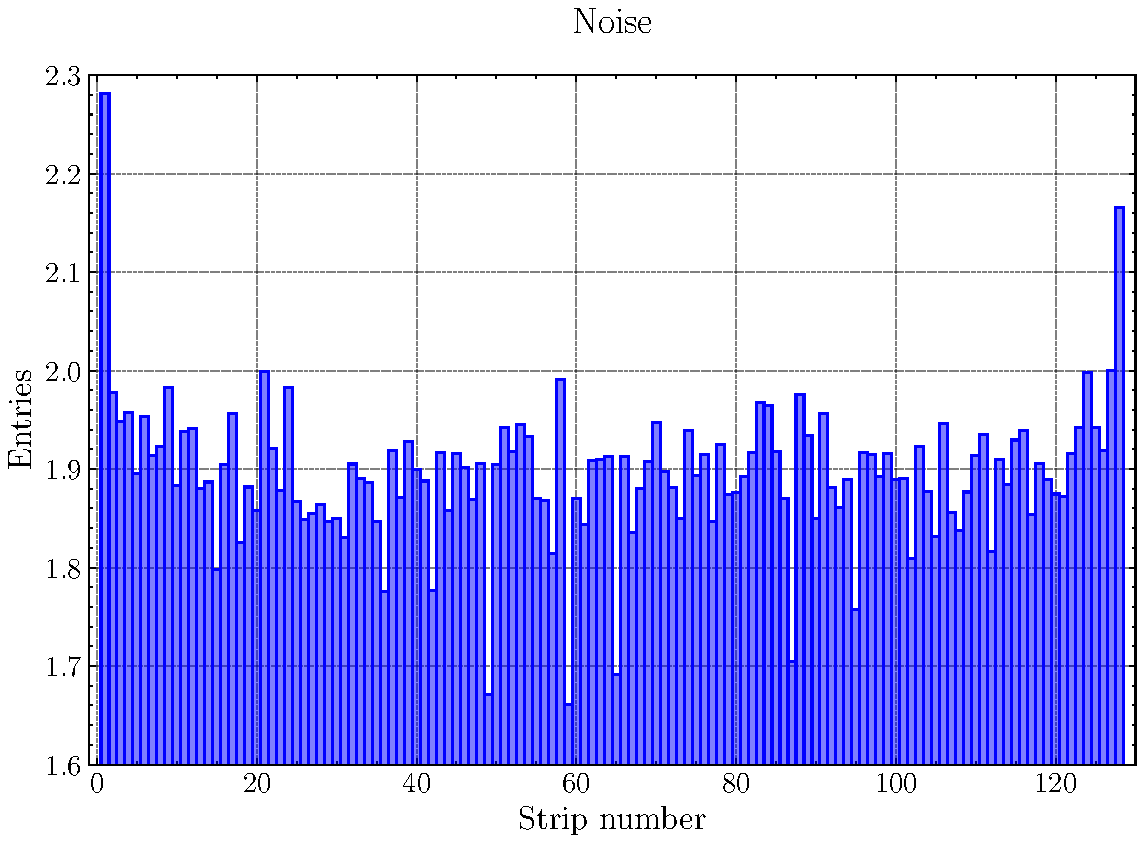
\includegraphics[scale=0.5]{graphs/noise.pdf}}
	\caption{Bar diagrams of the noise of the 128 individual strips.}
	\label{fig:noise}
\end{figure}

The electronic noise $\sigma(i)$ for each strip is derived through application of \cref{eq:noise}, which incorporates both the pedestals and common mode corrections. This noise parameter represents the fundamental resolution limit for signal detection in each channel.

\autoref{fig:pedestal} and \autoref{fig:noise} present the spatial distribution of pedestal and noise values across the detector array. Both parameters exhibit pronounced elevation near the chip periphery, because of the structure of the chip or the way the signal is
read out. 

The common mode shift distribution, displayed in \autoref{fig:shift}, demonstrates the expected Gaussian profile centered at zero. This confirms the stochastic nature of system-wide electronic fluctuations and validates the common mode correction methodology.

\begin{figure}[H]
       %\setkeys{Gin}{draft=false}
	\centering
	\fcolorbox{black}{white}{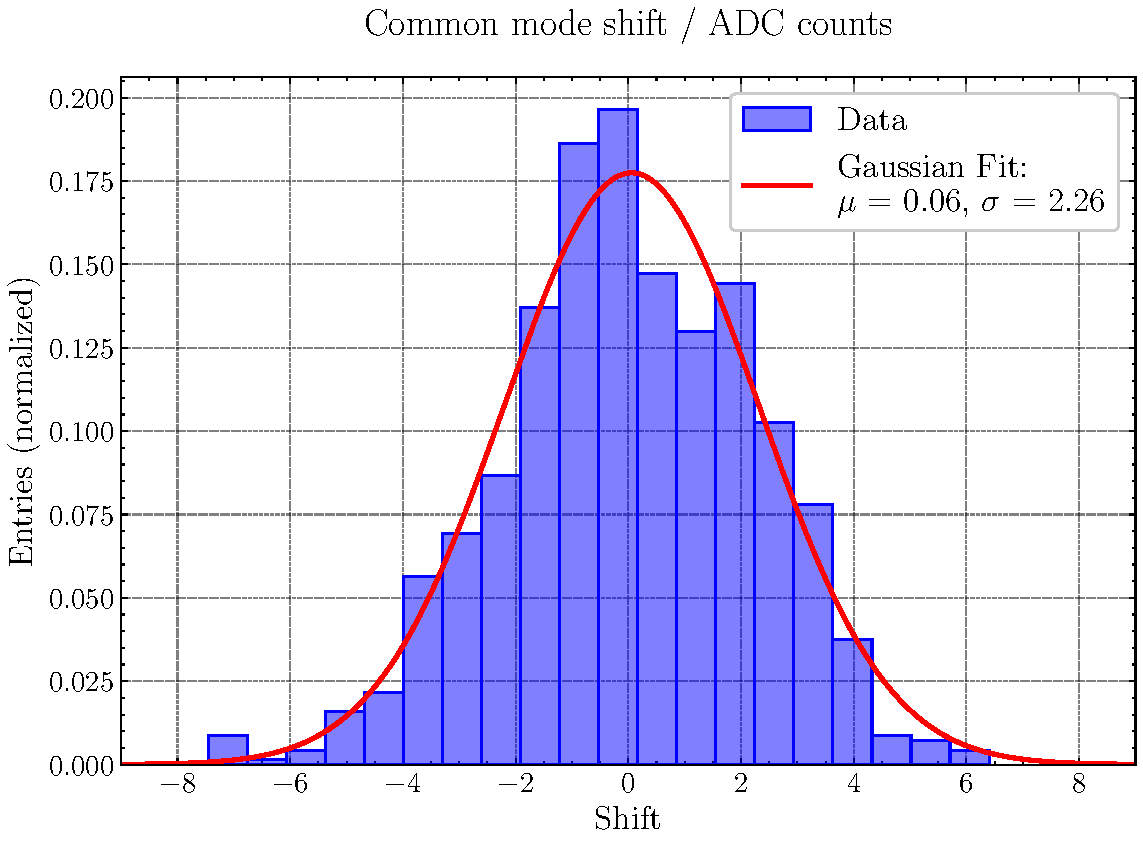
\includegraphics[scale=0.5]{graphs/shift.pdf}}
	\caption{Common mode shift measured during the pedestal run.}
	\label{fig:shift}
\end{figure}
%----------------------------------------------------%
\section{Calibration measurements}

\autoref{fig:optdelay} shows the ADC counts depending on the delay of the chip readout: the maximum signal amplitude occurs at 64 ns delay, establishing this as the optimal setting for subsequent experimental measurements. 

Following timing optimization, charge injection calibration was performed across five representative channels. The resulting calibration curves, presented in \autoref{fig:calibmeas}, demonstrate the relations between injected charge and ADC response. As one can see in \autoref{fig:calib0volt}, an additional curve at 0 V is recorded for channel 80 and compared to the regular curve of this channel.

\begin{figure}[H]
       %\setkeys{Gin}{draft=false}
	\centering
	\fcolorbox{black}{white}{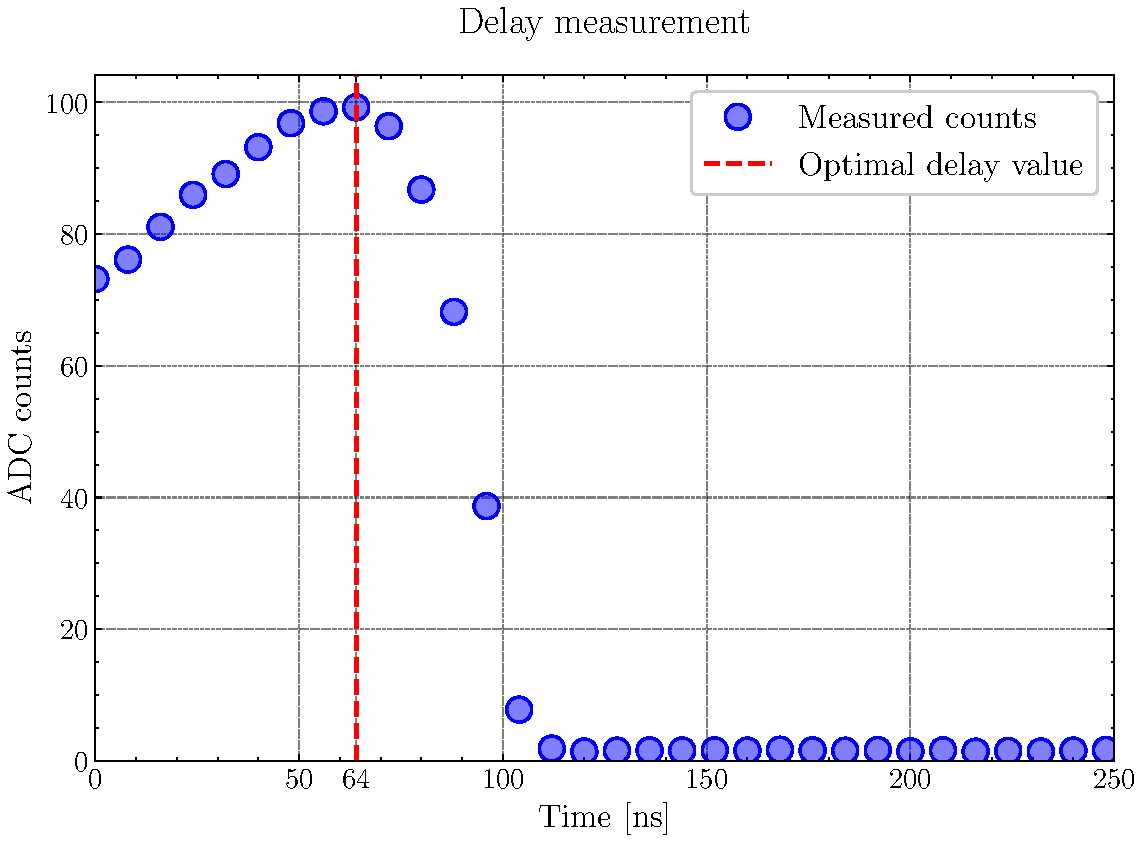
\includegraphics[scale=0.5]{graphs/optDelay.pdf}}
	\caption{Strength of the signal as function of the delay time. The red line highlights the optimal one (64 ns).}
	\label{fig:optdelay}
\end{figure}

\begin{figure}[H]
       %\setkeys{Gin}{draft=false}
	\centering
	\fcolorbox{black}{white}{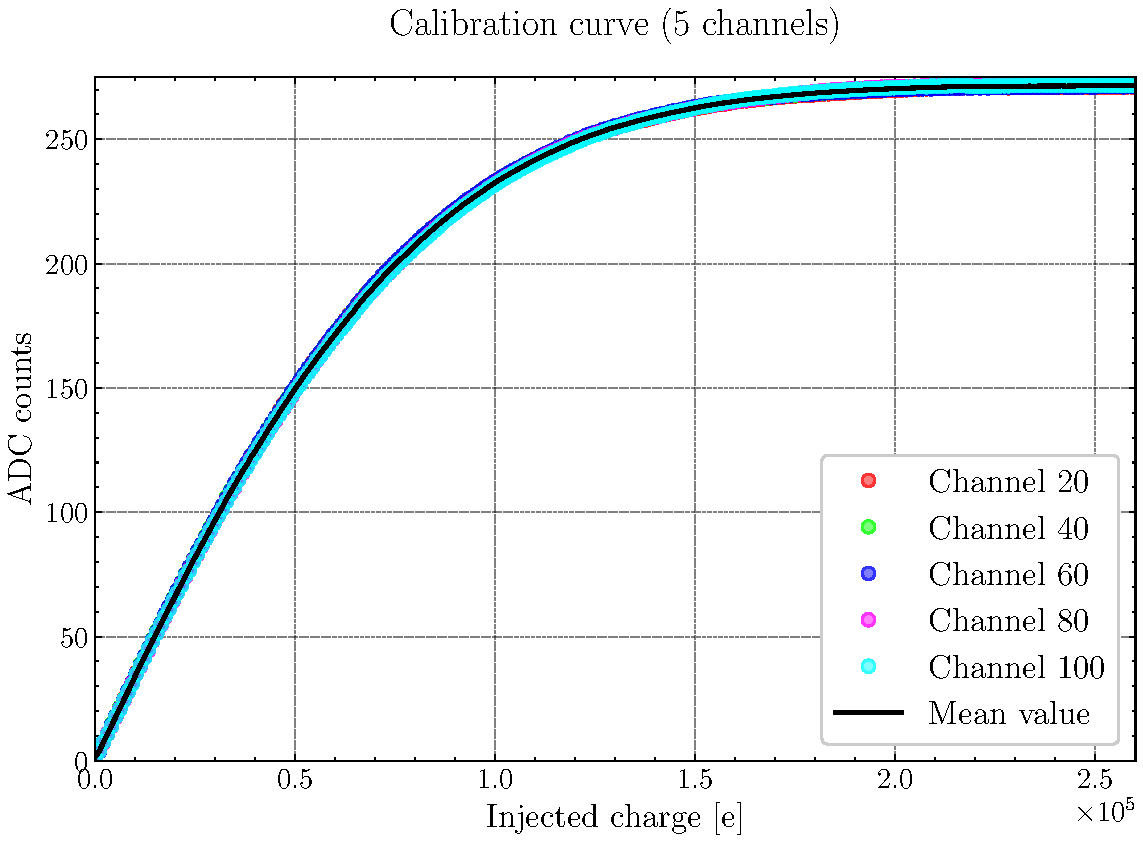
\includegraphics[scale=0.5]{graphs/calibMeas.pdf}}
	\caption{Calibration curve of five channels.}
	\label{fig:calibmeas}
\end{figure}

\begin{figure}[H]
       %\setkeys{Gin}{draft=false}
	\centering
	\fcolorbox{black}{white}{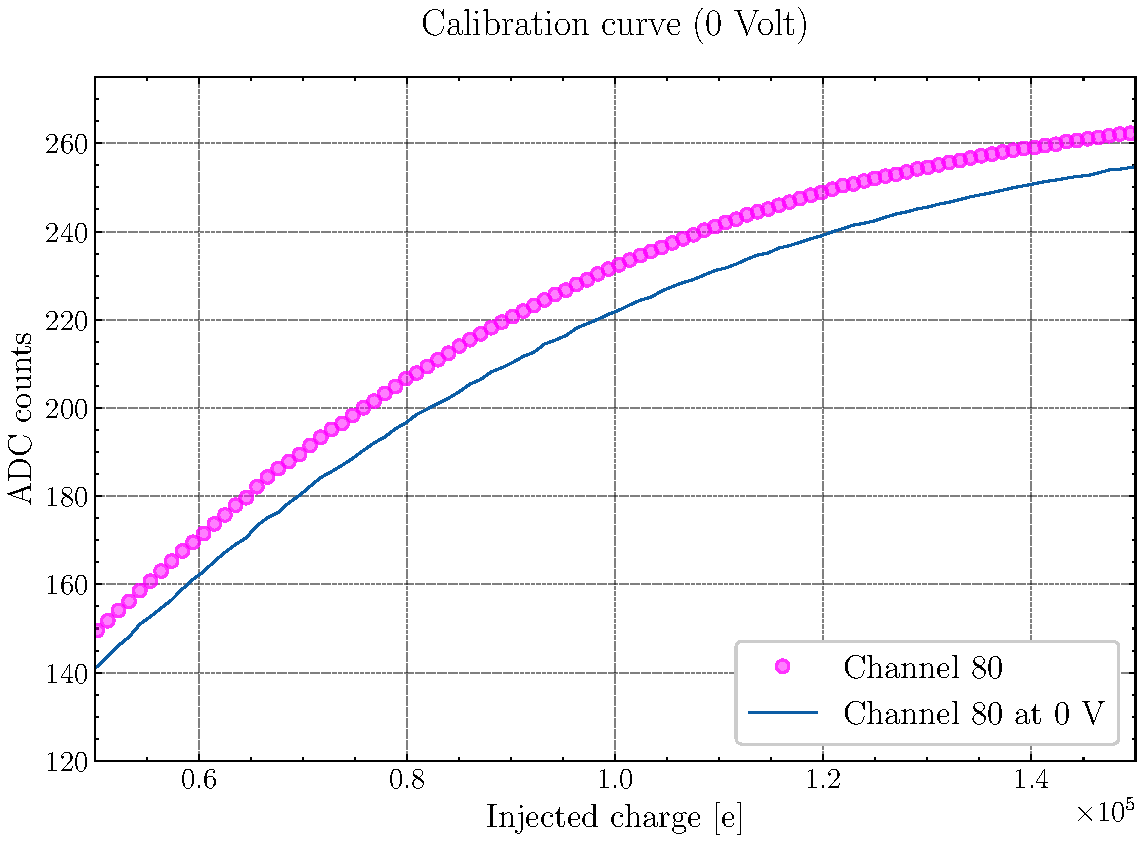
\includegraphics[scale=0.5]{graphs/calib0Volt.pdf}}
	\caption{Detailed view of channel 80 at 0 V.}
	\label{fig:calib0volt}
\end{figure}

As showed in \autoref{fig:calibmeas}, the calibration profiles exhibit remarkable consistency across all channels. The average of the five channels reveals a systematic voltage dependence: measurements at 0 V bias yield lower calibration values compared to those above the depletion voltage. This expected behaviour stems from the reduced depletion region width at zero bias, which decreases charge collection efficiency and thereby reduces registered ADC counts, as confirmed in \autoref{fig:calib0volt}.

To quantitatively characterize the charge response, a fourth-order polynomial was fitted to the mean ADC values:
\begin{equation}
    Q(\text{ADC}) = a \cdot \text{ADC}^4 + b \cdot \text{ADC}^3 + c \cdot \text{ADC}^2 + d \cdot \text{ADC} + e \label{eq:fit}
\end{equation}
where $Q$ represents the injected charge. Optimal fitting required restricting the analysis to the domain below 250 ADC counts, as higher values introduced non-linear effects that reduce model accuracy. The resulting calibration function is presented in \autoref{fig:polyfit}.

\begin{figure}[H]
       %\setkeys{Gin}{draft=false}
	\centering
	\fcolorbox{black}{white}{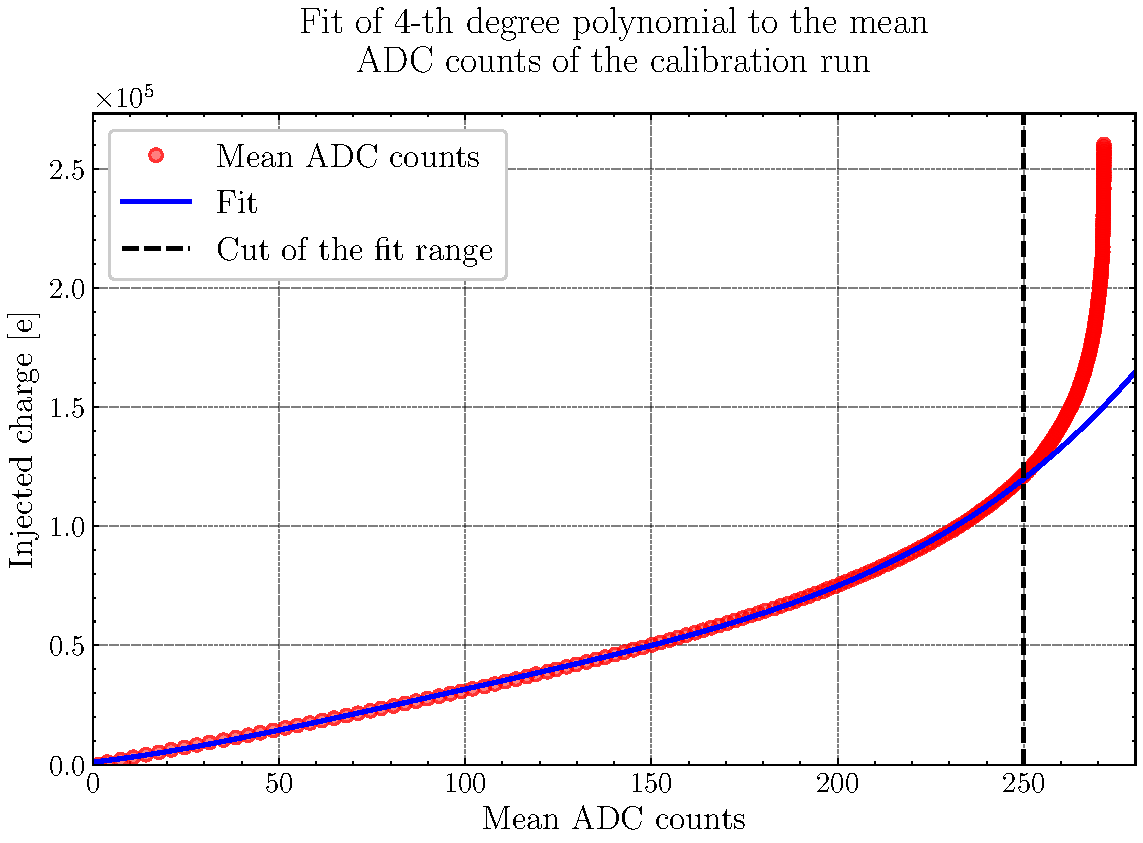
\includegraphics[scale=0.5]{graphs/polyFit.pdf}}
	\caption{Injected charge and corresponding ADC counts. A forth degree polynomial function is fitted to the data.}
	\label{fig:polyfit}
\end{figure}

The fit yields the following coefficients:
\begin{align*}
a &= (5.3 \pm 0.4) \times 10^{-5}  \text{e} \\
b &= (-1.91 \pm 0.21) \times 10^{-2}  \text{e} \\
c &= (2.7 \pm 0.4)  \text{e} \\
d &= (1.75 \pm 24) \times 10^{2} \text{e} \\
e &= (9.8 \pm 0.5) \times 10^{2}  \text{e}
\end{align*}

These coefficients together with \cref{eq:fit} now allow any ADC counts to be converted into an electric charge.
%----------------------------------------------------%
\section{Characteristics of the strip sensor}

Geometric parameters of the detector, particularly strip pitch and width, were determined through controlled laser excitation of the sensor. Prior to these measurements, precise temporal synchronization between the laser pulse and readout electronics was established. This synchronization was optimized by systematically varying the trigger delay while monitoring the resulting ADC counts. By definition, the optimal delay time produces the most intense signal, therefore, by looking at \autoref{fig:lasersync}, its value can be set to 110 ns.

\begin{figure}[H]
       %\setkeys{Gin}{draft=false}
	\centering
	\fcolorbox{black}{white}{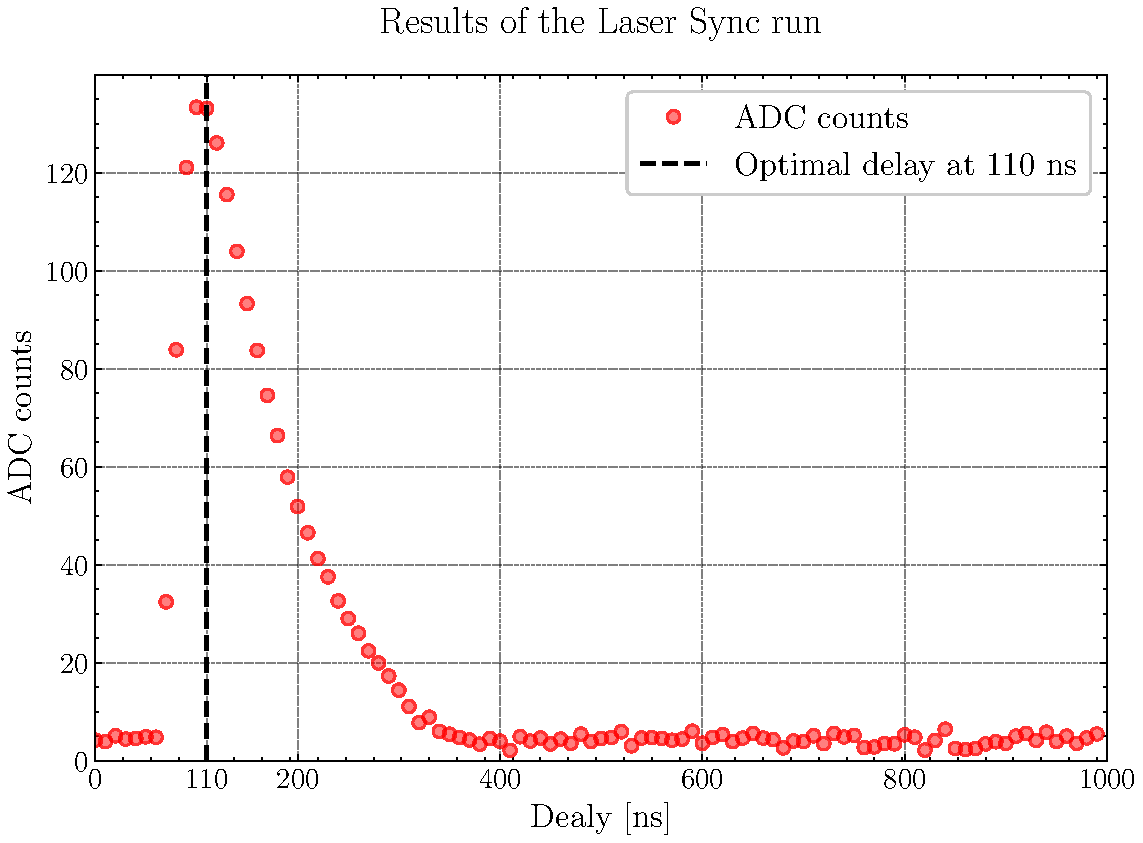
\includegraphics[scale=0.4]{graphs/laserSync.pdf}}
	\caption{Results of the \textit{laser sync} run.}
	\label{fig:lasersync}
\end{figure}

After laser-readout synchronization, the laser was translated across the detector surface in 10 \textmu m increments while recording ADC responses at each position. The resulting spatial profile of ADC counts is presented in \autoref{fig:bigheat} and \autoref{fig:smallheat}, revealing localized signal maxima corresponding to individual sensor strips.

\begin{figure}[H]
       %\setkeys{Gin}{draft=false}
	\centering
	\fcolorbox{black}{white}{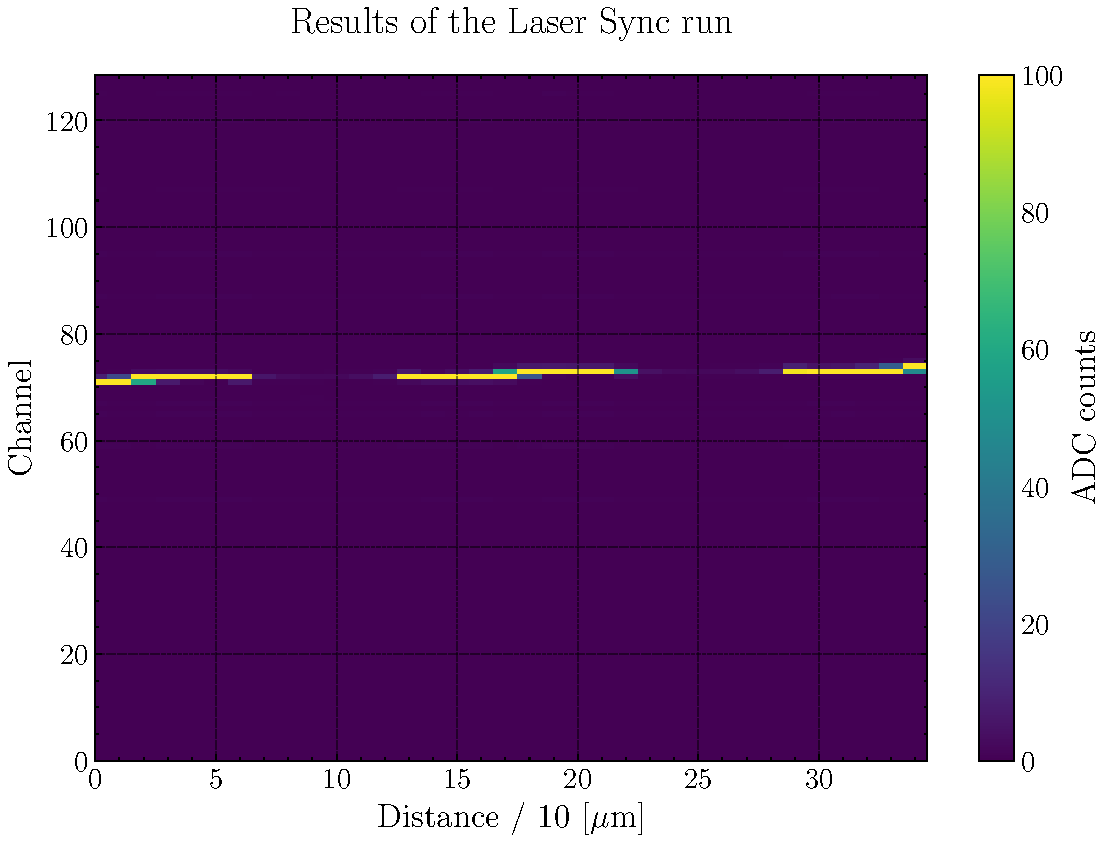
\includegraphics[scale=0.5]{graphs/bigHeatmap.pdf}}
	\caption{Heatmap of the signal strength of all the channels  depending on the laser position.}
	\label{fig:bigheat}
\end{figure}

\begin{figure}[H]
       %\setkeys{Gin}{draft=false}
	\centering
	\fcolorbox{black}{white}{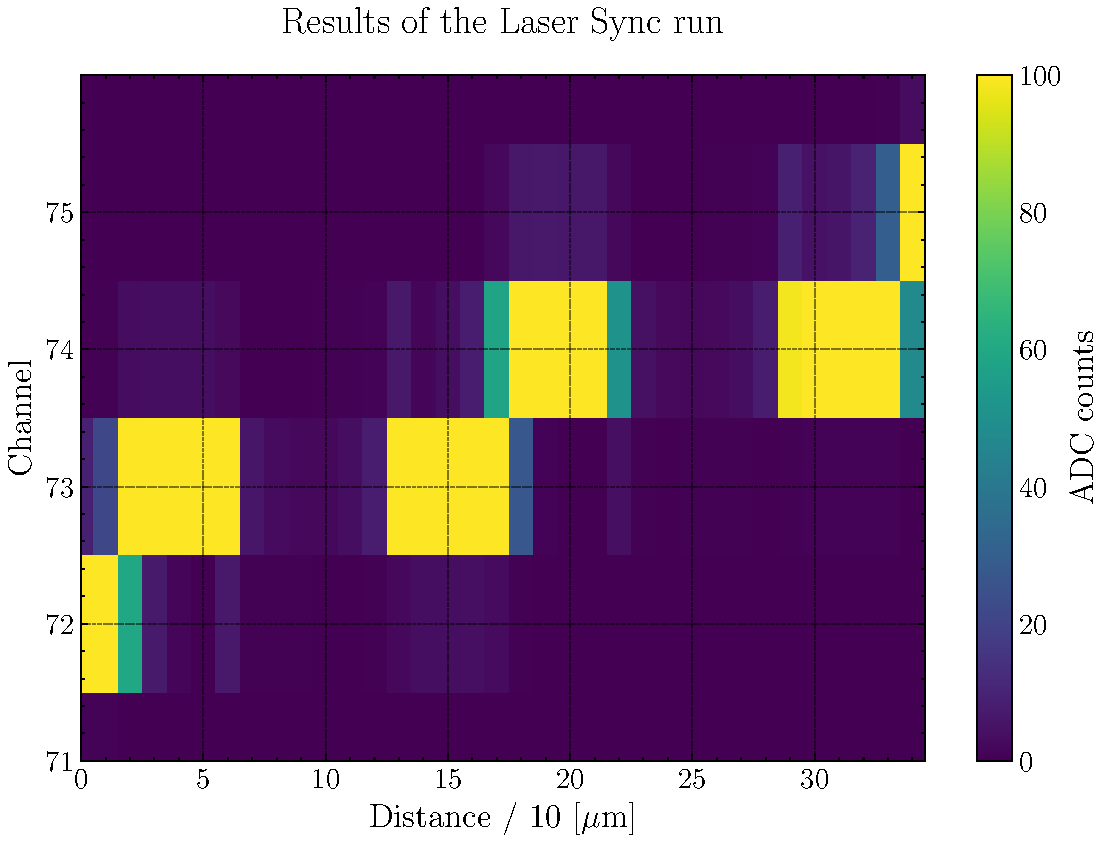
\includegraphics[scale=0.5]{graphs/smallHeatmap.pdf}}
	\caption{Heatmap of the signal strength of the affected channels (73, 74) depending on the laser position.}
	\label{fig:smallheat}
\end{figure}

\begin{figure}[H]
       %\setkeys{Gin}{draft=false}
	\centering
	\fcolorbox{black}{white}{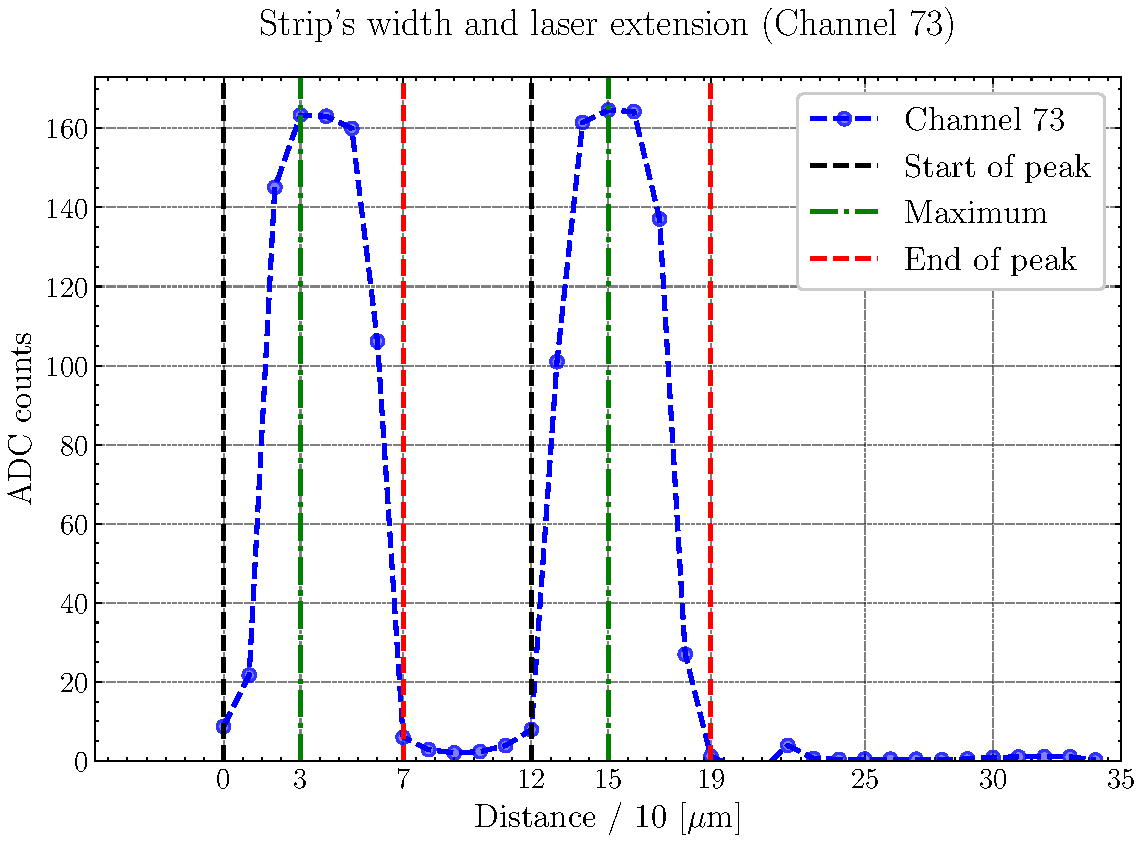
\includegraphics[scale=0.5]{graphs/width73.pdf}}
	\caption{Signal strength of channel 73 depending on the laser position.}
	\label{fig:73}
\end{figure}

Analysis of the spatial distribution identifies channels 73 and 74 as exhibiting pronounced signal peaks. The ADC responses from these channels (detailed in \autoref{fig:73} and \autoref{fig:74}) provide the strip pitch, by measuring the spatial separation between adjacent response maxima. The width of the laser beam follows from the distance between the minimum and maximum of a peak.

\begin{figure}[H]
       %\setkeys{Gin}{draft=false}
	\centering
	\fcolorbox{black}{white}{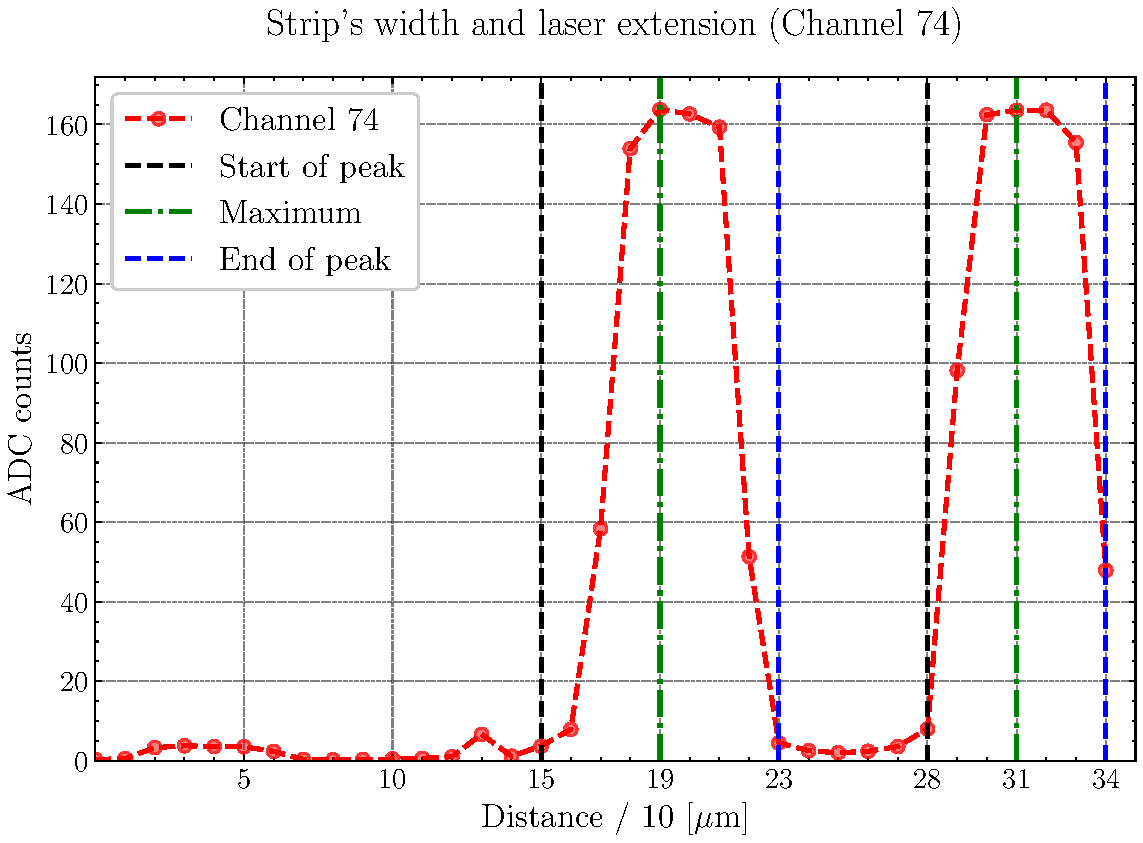
\includegraphics[scale=0.5]{graphs/width74.pdf}}
	\caption{Signal strength of channel 74 depending on the laser position.}
	\label{fig:74}
\end{figure}

The width of the strip is the distance between the two peaks; the extension of the laser can be estimated by the distance between the start of a peak and its maximum and the distance of two strips can be determined by comparing the position of the maxima
of two different channels. The pitch is then calculated as the sum of the distance between the strips and their width:
\begin{align*}
\text{width of strips} &= 150 - 30 \hspace{2pt}(\text{ch73}) = 310 - 190 \hspace{2pt}(\text{ch74}) = 120 \mu \text{m} \\
\text{laser extension} &= 150 - 120 \hspace{2pt}(\text{ch73}) = 310 - 280 \hspace{2pt}(\text{ch74}) = 30 \mu \text{m} \\
\text{distance of strips} &= 190\hspace{2pt}(\text{ch74}) - 150\hspace{2pt}(\text{ch73}) = 40 \mu \text{m} \\
\text{pitch} &= 120 - 40 = 160 \mu \text{m}
\end{align*}
%----------------------------------------------------%
\section{Charge Collection Efficiency}

In this part of the analysis, the charge collection efficiency (CCE) of the laser is determined in two ways: first, the laser is used to excite the sensor; second, while a $\beta^{-}$ source is employed later.

\subsection{CCEL (laser)}

When using the laser to excite the sensor, in first place it necessary to determine which channel the laser is focused on. By plotting a heatmap of the ADC counts for each channel, we can see that the laser was focused on channel 72, \autoref{fig:bigvolt} and \autoref{fig:smallvolt}.
\begin{figure}[H]
       %\setkeys{Gin}{draft=false}
	\centering
	\fcolorbox{black}{white}{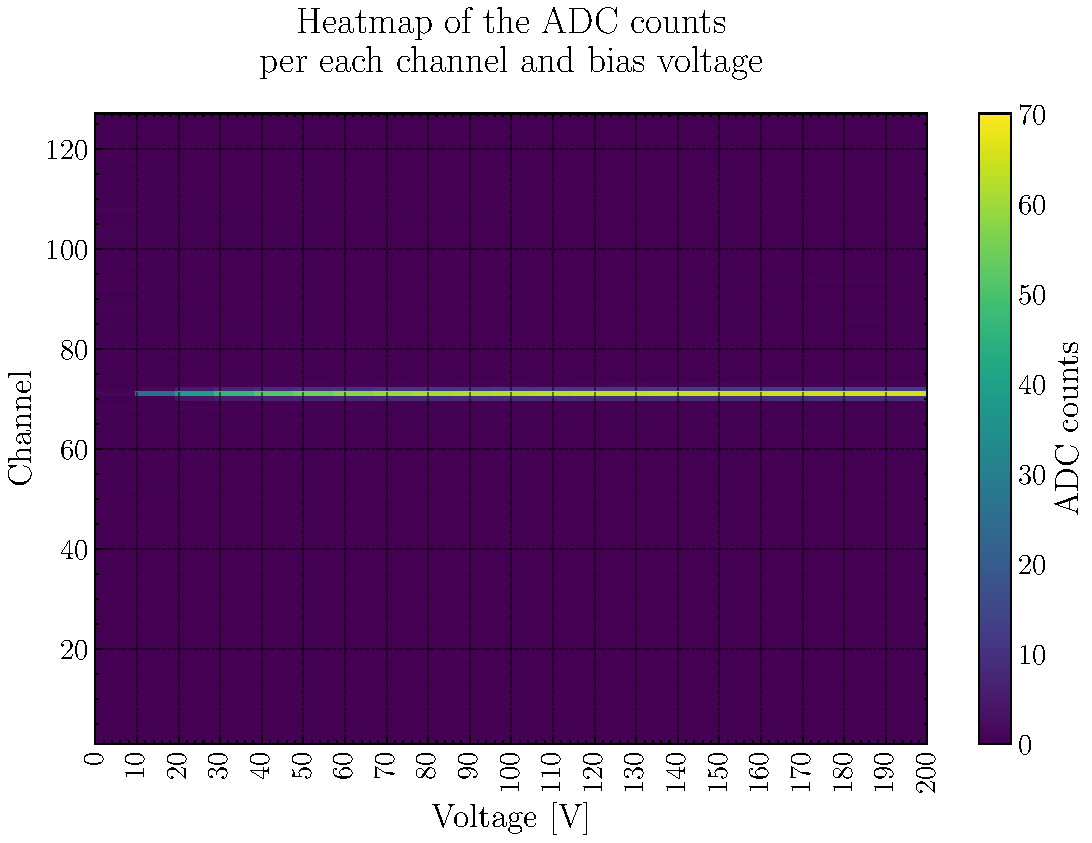
\includegraphics[scale=0.4]{graphs/bigVoltage.pdf}}
	\caption{Heatmap showing the ADC counts of each channel and bias voltage.}
	\label{fig:bigvolt}
\end{figure}

\begin{figure}[H]
       %\setkeys{Gin}{draft=false}
	\centering
	\fcolorbox{black}{white}{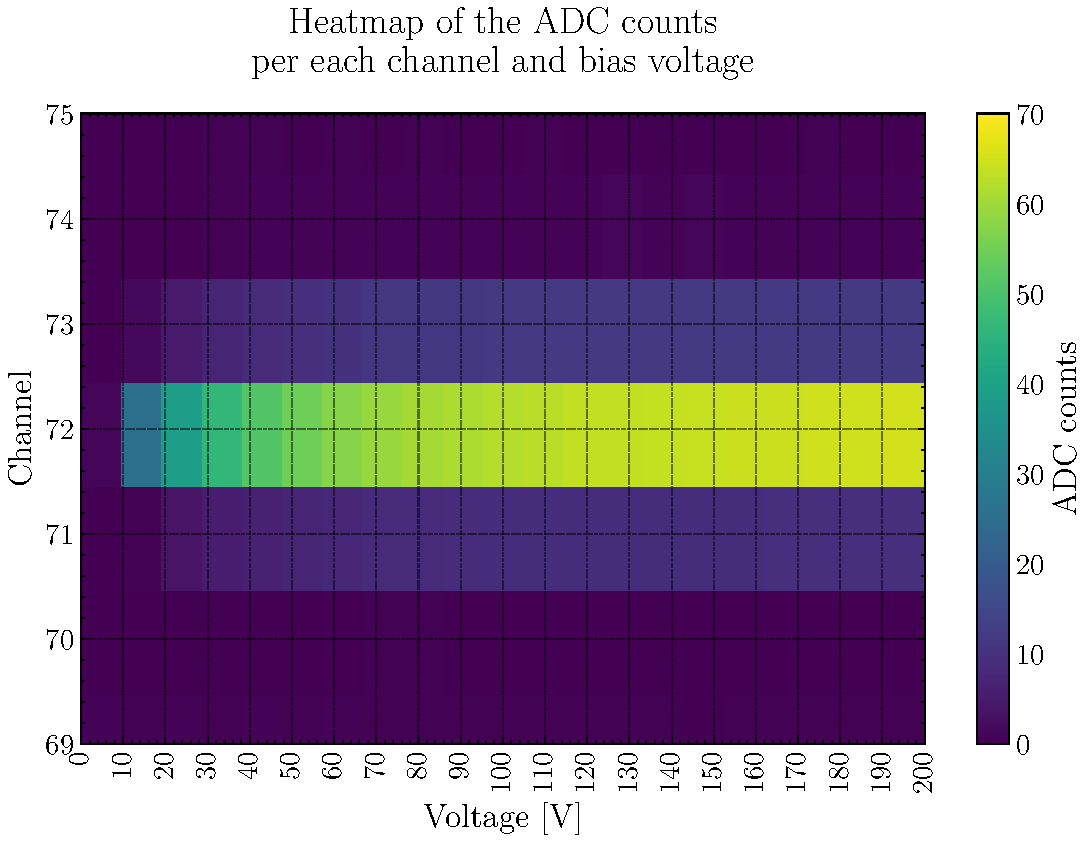
\includegraphics[scale=0.4]{graphs/smallVoltage.pdf}}
	\caption{Zoomed heatmap showing the ADC counts of channel 72 and bias voltage.}
	\label{fig:smallvolt}
\end{figure}

To determine the laser penetration depth, \cref{eq:fitdepl} was fitted to the data from channel 72. This required normalization of ADC values relative to their maximum expected response. Theoretical models predict a constant plateau in ADC counts for bias voltages exceeding the depletion voltage ($U_{\text{dep}}$). However, observed plateau regions exhibited minor non-constant behavior due to experimental imperfections. To address this, normalization was performed in regard to the first value of the plateau. The fitting procedure was performed in the range $0  \text{V} < U < 80  \text{V}$. Within this domain, the depletion voltage $U_{\text{dep}} = 80$ V was maintained as a fixed parameter, so this yielded a penetration depth of:
\[
a = (252 \pm 72)  \mu\text{m}
\]

\begin{figure}[H]
       %\setkeys{Gin}{draft=false}
	\centering
	\fcolorbox{black}{white}{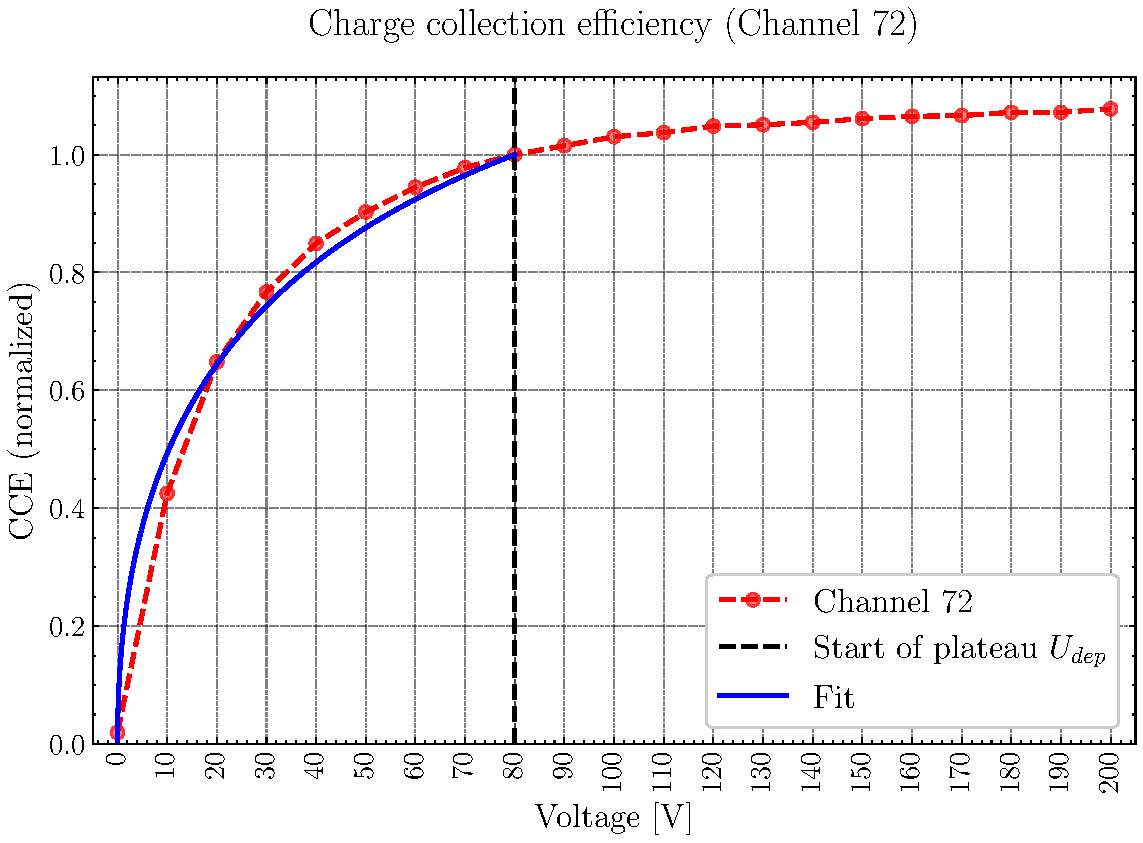
\includegraphics[scale=0.5]{graphs/channel72.pdf}}
	\caption{Charge collection efficiency of channel 72.}
	\label{fig:cce72}
\end{figure}

\subsection{CCEQ (beta source)}

Analogously to the previous analysis step, the measurement of the CCE with a $\beta^{-}$ source yields a plot of the ADC counts in dependence of the bias voltage. The mean value across all detected clusters was subsequently calculated to determine charge collection efficiency. This value underwent normalization identical to the laser-based measurement protocol. The resultant characteristic curve depicting system response is presented in \autoref{fig:beta}.

In \autoref{fig:betalaser} we can see that the curve obtained through laser excitation exhibits an earlier response to increasing bias potential compared to the radioactive source method. Both profiles converge completely beyond the depletion voltage threshold. This behavior indicates reduced detection efficiency for charged particles at lower voltages compared to laser photons. When operating above the critical depletion voltage, this discrepancy becomes negligible as both measurement techniques demonstrate identical charge collection characteristics.

\begin{figure}[H]
       %\setkeys{Gin}{draft=false}
	\centering
	\fcolorbox{black}{white}{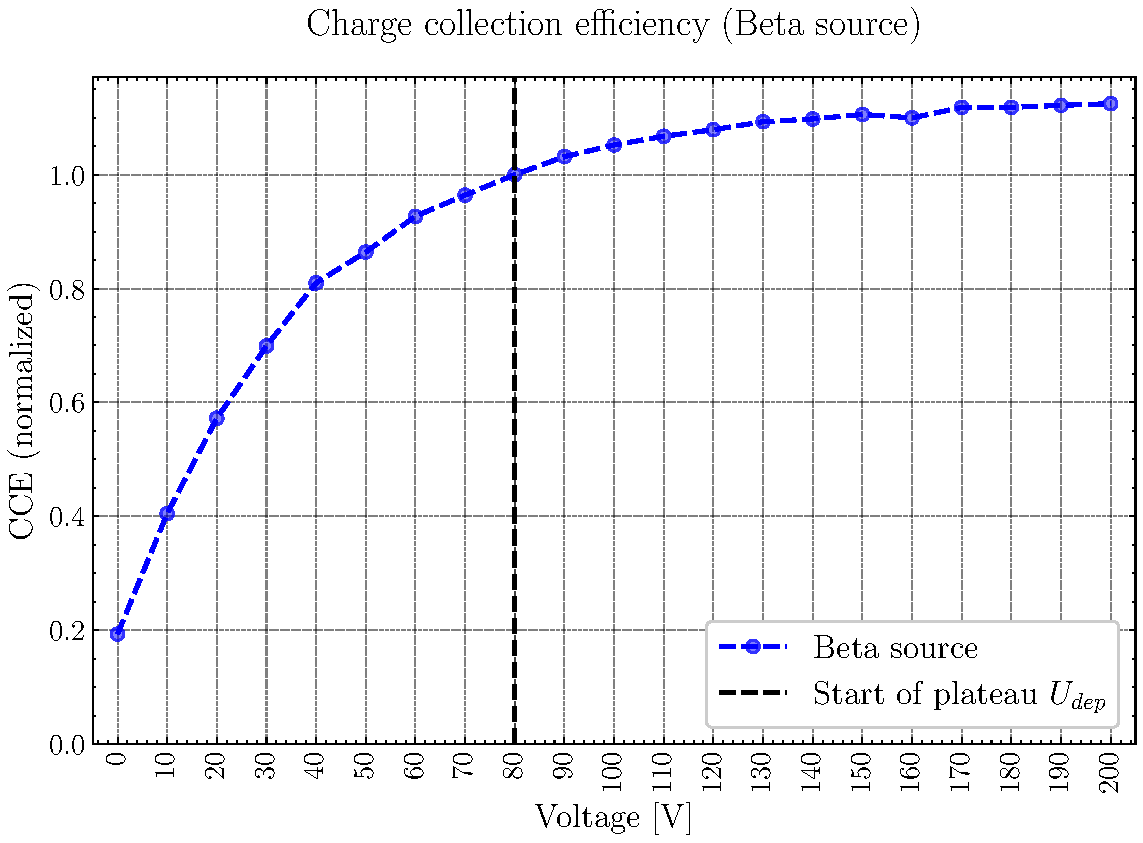
\includegraphics[scale=0.4]{graphs/betaSource.pdf}}
	\caption{Charge collection efficiency determined via the $\beta^{-}$ source.}
	\label{fig:beta}
\end{figure}

\begin{figure}[H]
       %\setkeys{Gin}{draft=false}
	\centering
	\fcolorbox{black}{white}{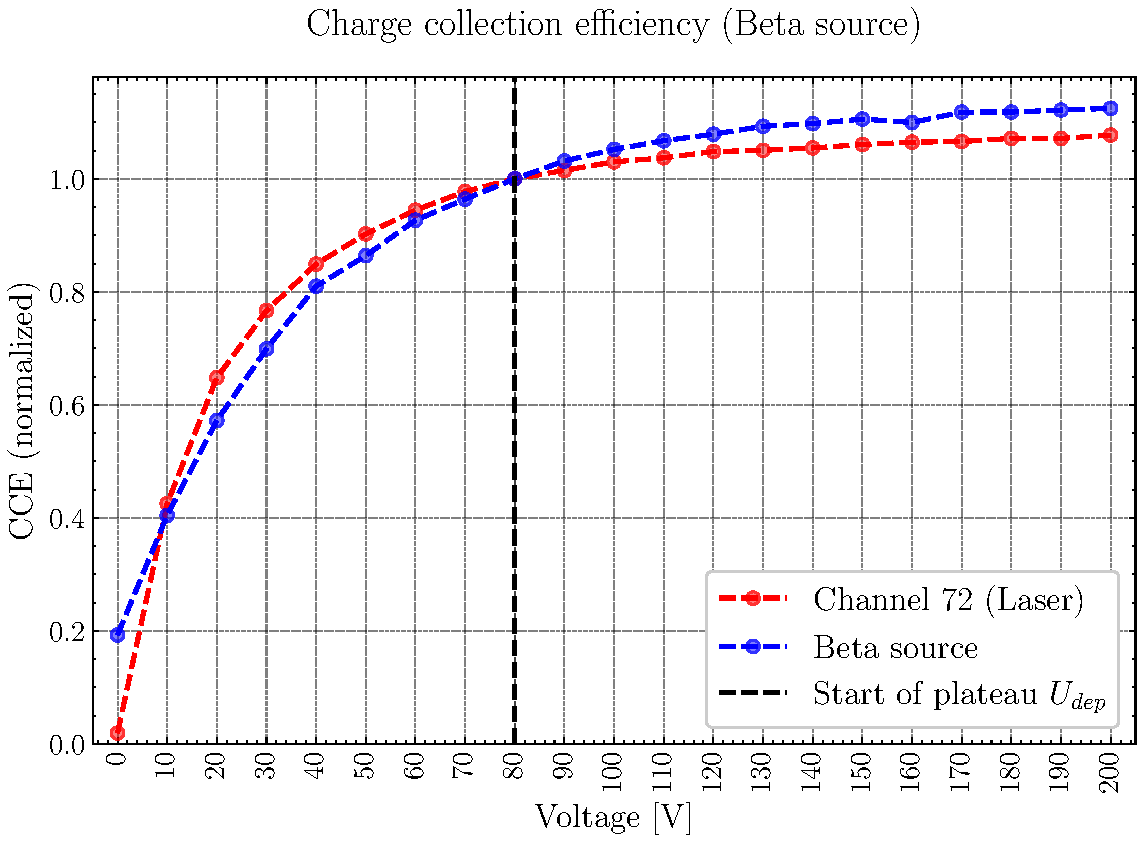
\includegraphics[scale=0.4]{graphs/betaLaserSource.pdf}}
	\caption{Comparison of the charge collection efficiency determined via the laser and
the $\beta^{-}$ source, respectively.}
	\label{fig:betalaser}
\end{figure}
%----------------------------------------------------%
\section{Large source scan}

For the last measurement, 1,000,000 events are recorded in the $\beta^{-}$ source configuration. Two relevant quantities are recorded and plotted in \autoref{fig:cluster} and \autoref{fig:cluchans}: the number of clusters per event and the the number of channels per cluster. Since there is a possibility that more than one channel is fired within the same cluster, one can conclude that the trajectory of electrons is not always perpendicular to the plane of the strips.
\begin{figure}[H]
       %\setkeys{Gin}{draft=false}
	\centering
	\fcolorbox{black}{white}{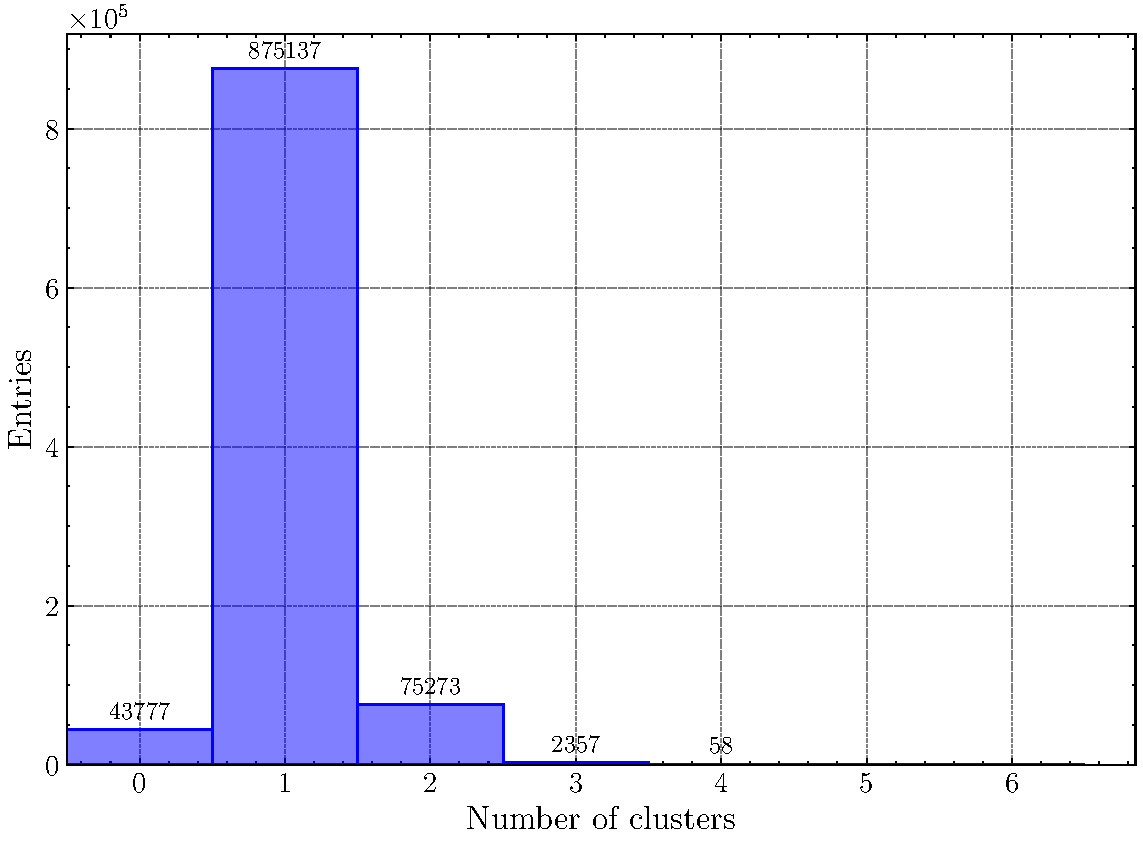
\includegraphics[scale=0.4]{graphs/cluster.pdf}}
	\caption{Number of clusters per event.}
	\label{fig:cluster}
\end{figure}

\begin{figure}[H]
       %\setkeys{Gin}{draft=false}
	\centering
	\fcolorbox{black}{white}{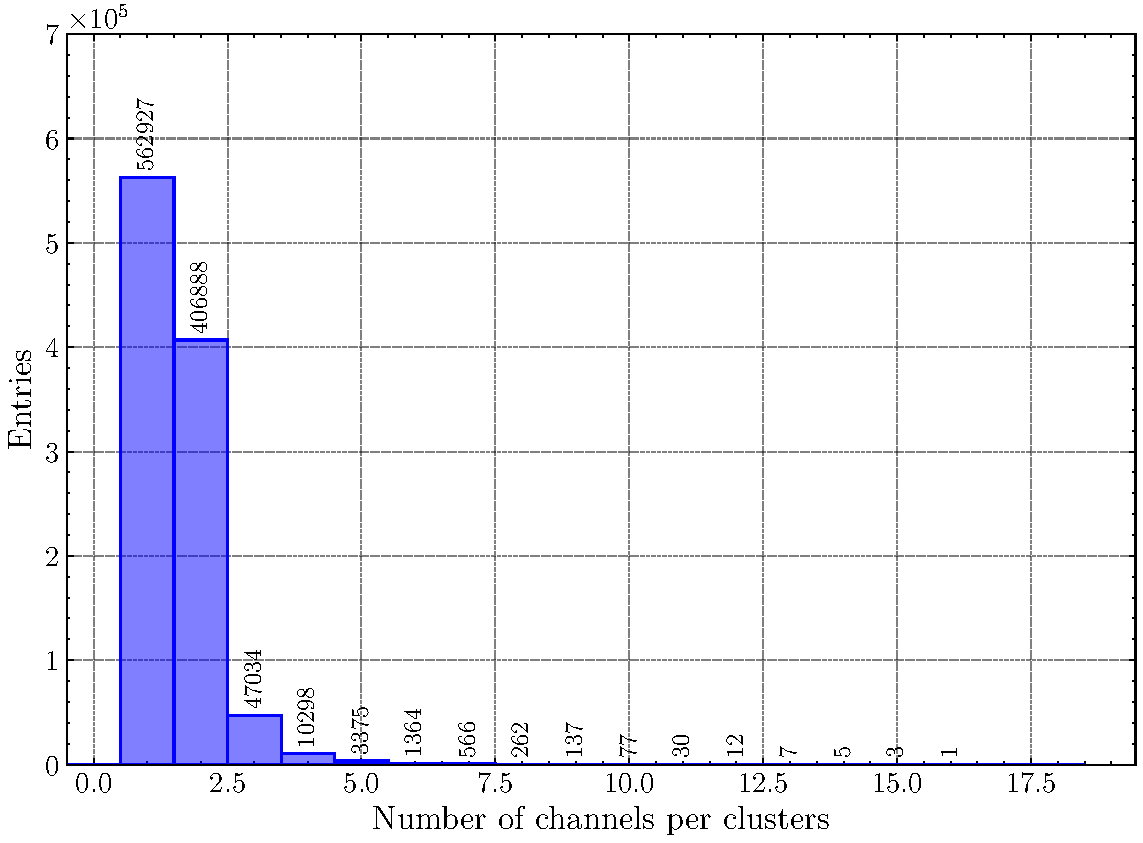
\includegraphics[scale=0.4]{graphs/cluchans.pdf}}
	\caption{Number of channels per cluster.}
	\label{fig:cluchans}
\end{figure}

Following, the plot of the distribution of the number hits for each channel during the run, in \autoref{fig:hitmap}. Note: the central channels are the ones being hit most frequently since
they are aligned with the radioactive source.

\begin{figure}[H]
       %\setkeys{Gin}{draft=false}
	\centering
	\fcolorbox{black}{white}{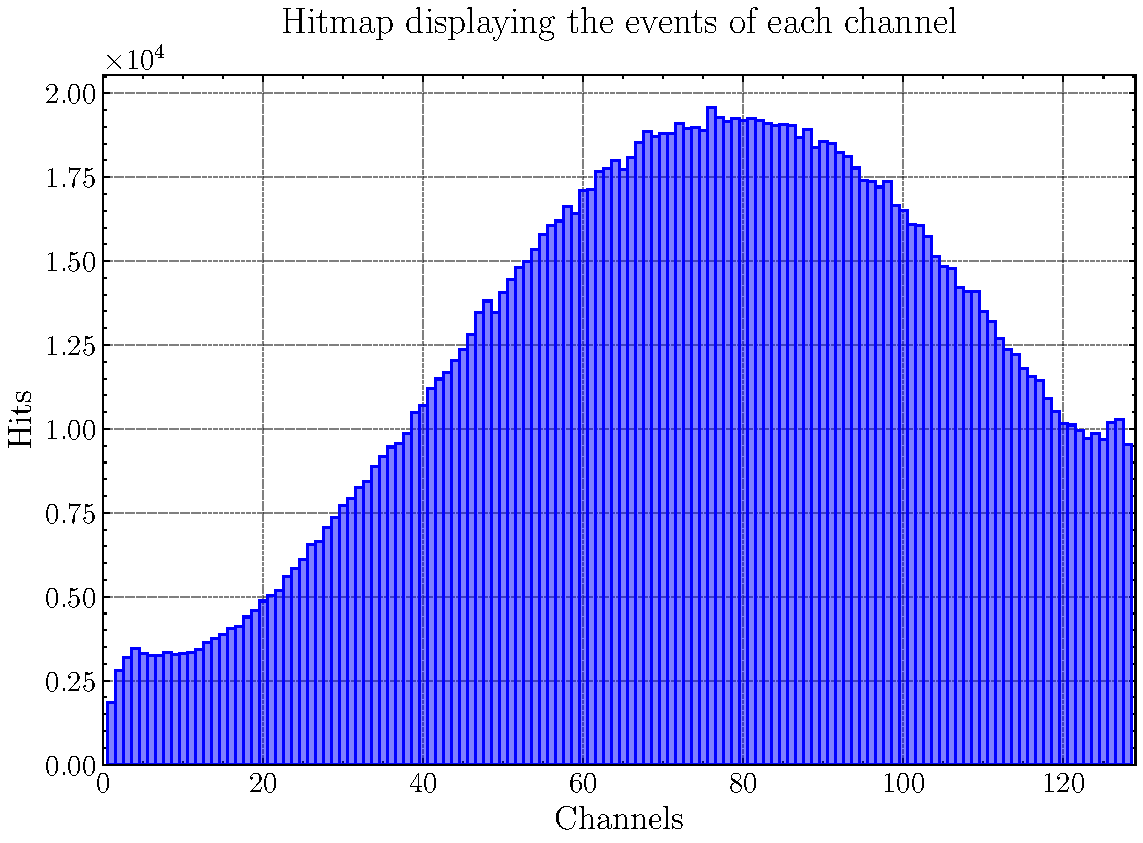
\includegraphics[scale=0.5]{graphs/hitmap.pdf}}
	\caption{Hitmap displaying the events of each channel.}
	\label{fig:hitmap}
\end{figure}

The spatial hit distribution exhibits pronounced centrality, with the highest event density occurring near the sensor's geometric center and diminishing toward peripheral regions. Subsequently, statistical distributions of both raw ADC measurements and derived energy values were computed. To transform ADC counts into physical energy values, the conversion relationship established during calibration, \cref{eq:fit}, was first applied to obtain equivalent charge pulses. These pulse magnitudes were then converted to energy units using the fundamental silicon ionization energy of 3.6 eV required to create an electron-hole pair. The resulting distributions for both ADC counts and energy spectra are presented collectively in \autoref{fig:energydistrib}.

\begin{figure}[H]
       %\setkeys{Gin}{draft=false}
	\centering
	\fcolorbox{black}{white}{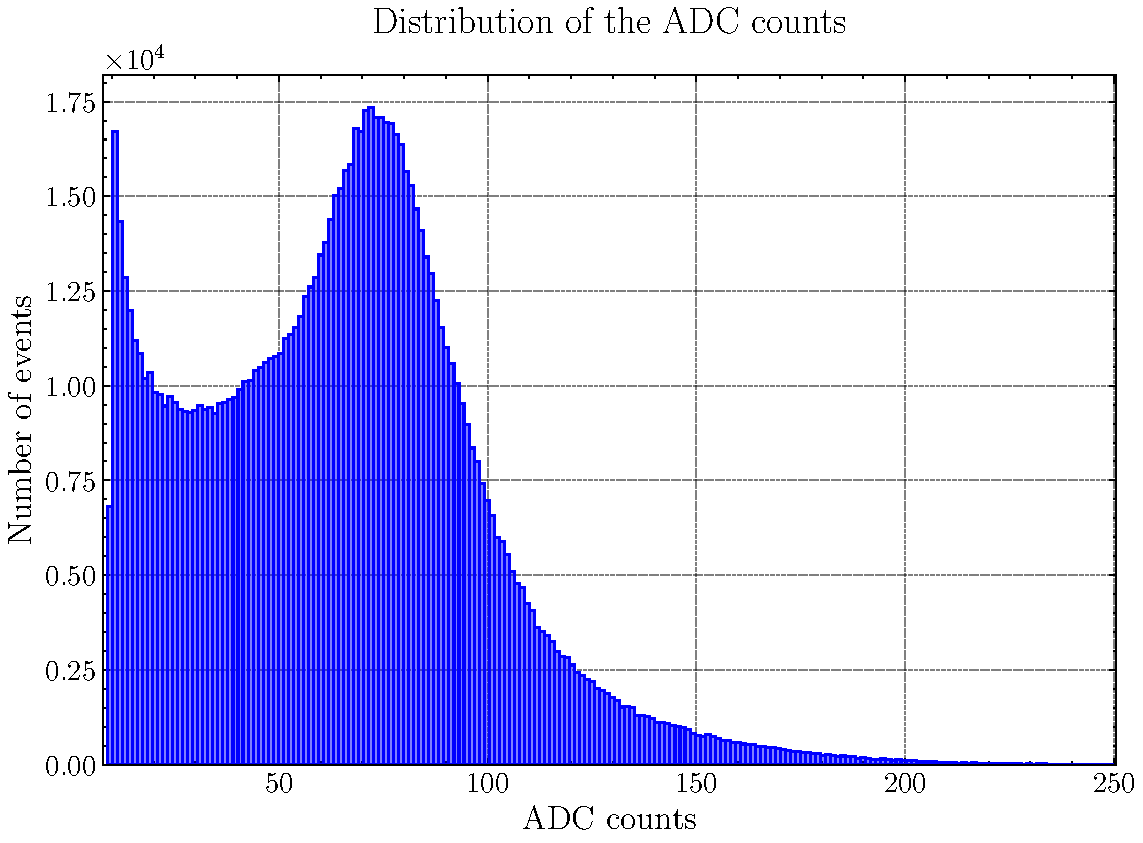
\includegraphics[scale=0.4]{graphs/ADCdistrib.pdf}}
	\caption{Distribution of the ADC counts.}
	\label{fig:ACD}
\end{figure}

\begin{figure}[H]
       %\setkeys{Gin}{draft=false}
	\centering
	\fcolorbox{black}{white}{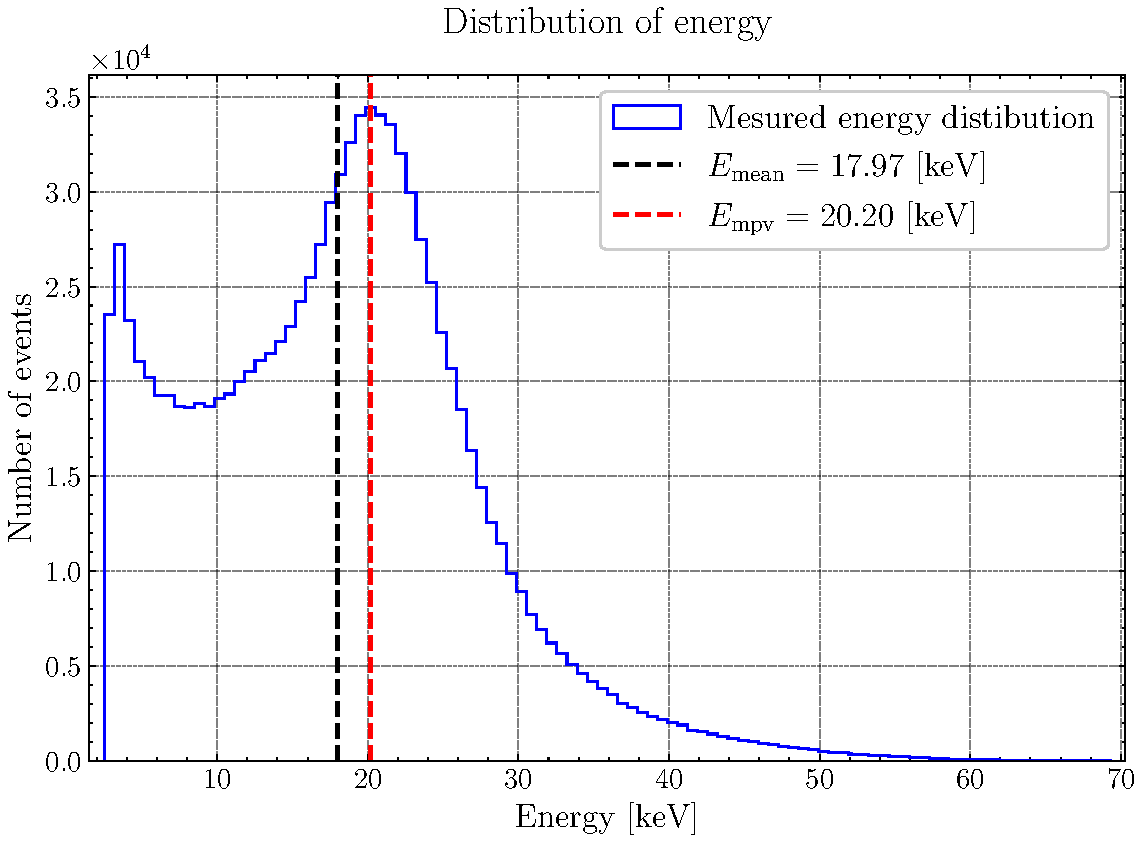
\includegraphics[scale=0.4]{graphs/ENERGYdistrib.pdf}}
	\caption{Energy distribution of the $\beta^{-}$ source.}
	\label{fig:energydistrib}
\end{figure}

Analysis of the spectral energy distribution enables derivation of characteristic energy parameters for the $\beta^{-}$ source:
\begin{align*}
E_{\text{mean}} &= 17.97  \hspace{2pt}\text{keV} \\
E_{\text{mpv}} &= 20.20  \hspace{2pt}\text{keV}
\end{align*}
where $E_{\text{mpv}}$ denotes the most probable energy (peak value) and $E_{\text{mean}}$ represents the mean energy.
%----------------------------------------------------%
